\section*{\color{olive}Ejercicio 2: C\'alculo y simulaci\'on de una funci\'on transferencia de tensi\'on}

\begin{figure}[H] %!ht
 \begin{center}
    \begin{circuitikz}[american]
    \draw (0,3) to[sV,v=$V_{in}$] (0,0) % The voltage source
(0,3)  to[short] (1,3) to[R, l2_=$R_G$ and $50\Omega$] 
(2,3)  to[short] (3,3) to[C=$C_{in}$] (4,3) to[short] (5.5,3) 
%to[R=$R_G$]  (2,3)  to[short] (3,3) to[C=$c_{in}$] (4,3) to[short] (5.5,3) 
(6,3) node[npn]{}
(0,0) to[short] (6,0) to[R=$R_E$] (6,2.5)
(4.5,0) to[R=$R_2$] (4.5,3) to[R=$R_1$] (4.5,6) to[short] (6,6) to[R=$R_C$] (6,3.5)
 to[C=$C_{out}$] (9,3.5) node[anchor=west] {OUT} (9,3.5)
 to[R=$R_L$] (9,0) to[short] (6,0)
(7.5,0) to[pC=$C_E$] (7.5,2.5) to[short] (6,2.5)
(4.5,6)  to[V, v=$V_{cc}$] (0,6) node[ground]{}
(2.5,3) node[anchor=south] {IN} 
(4.5,0) node[ground]{};
    \end{circuitikz}
    \caption{Circuito con un transistor NPN BC547B, para el cual se obtiene la funci\'on transferencia.}
	\label{circ2}
\end{center}
\end{figure}


Siendo
%\begin{itemize}
%\item $ R_1 = 100k\Omega$
%\item $ R_2 = 27k\Omega$
%\item $ R_C = 11.2k\Omega$
%\item $ R_E = 3k\Omega$
%\item $ R_L = 10k\Omega$
%\item $ C_{in} = 20nF$
%\item $ C_{out} = 10nF$
%\item $ C_E = 2\mu F$
%\end{itemize}

\begin{multicols}{4}
\begin{itemize}
\item $ R_1 = 100k\Omega$
\item $ R_2 = 27k\Omega$
\end{itemize}
\columnbreak
\begin{itemize}
\item $ R_C = 11.2k\Omega$
\item $ R_L = 10k\Omega$
\end{itemize}
\columnbreak
\begin{itemize}
\item $ R_E = 3k\Omega$
\item $ C_E = 2\mu F$
\end{itemize}
\columnbreak
\begin{itemize}
\item $ C_{in} = 20nF$
\item $ C_{out} = 10nF$
\end{itemize}
\end{multicols}


\subsection*{\color{orange} C\'alculo de la funci\'on transferencia de tensi\'on}

Para calcular la funci\'on transferencia de tensi\'on del circuito \ref{circ2}, se utiliza el modelo h\'ibrido $\pi$ como circuito equivalente del transistor NPN en peque\~na se\~nal, pasivando la fuente de tensi\'on cont\'inua. Adem\'as, a muy bajas frecuencias se considera que los capacitores se comportan como cortocircuitos. El siguiente circuito es el equivalente correspondiente al circuito \ref{circ2}:

\begin{figure}[H]%!ht
 \begin{center}
    \begin{circuitikz}[american]
    \draw (0,1.5) to[sV,v=$V_{in}$] (0,0) % The voltage source
(0,1.5) to[R=$R_G$] (0,3)
(2,0) to[R=$R_1$] (2,3)
(4,0) to[R=$R_2$] (4,3)
(6,0) to[R=$R_{\pi}$] (6,3)
(8,3) to[cI=$I_1$] (8,0)
(10,0) to[R=$R_0$] (10,3)
(12,0) to[R=$R_C$] (12,3)
(14,0) to[R=$R_L$] (14,3)
	
(0,0) to[short] (14,0)
(0,3) to[short] (6,3)
(8,3) to[short] (14,3)
(7,0) node[ground]{}
(1,3) node[anchor=south] {IN} 
(14,3) node[anchor=west] {OUT};
    \end{circuitikz}
    \caption{Circuito equivalente empleado para el c\'alculo de la funci\'on transferencia de tensi\'on.}
	\label{circ22}
\end{center}
\end{figure}

En el gr\'afico anterior, siendo:
$$I_1 = \beta \cdot i_b$$
con $i_b$ la corriente que circula por la resistencia denominada $R_{\pi}$.

A partir del circuito \ref{circ22}, surge que:
\begin{equation}\frac{V_{OUT}}{V_{IN}} = \frac{\left( R_0 // R_C // R_L\right) \beta}{ R_{\pi}} = \frac{R_L \cdot (R_0 + R_C) \cdot \beta}{R_{\pi} \cdot (R_0 R_C R_L + R_0 + R_C)} \label{ec1} \end{equation}

A partir de la simulaci\'on, medimos la impedancia de salida del circuito de la figura \ref{circ2} y obtuvimos el valor de $R_0$ del transistor NPN BC547B:\\
$R_0 = 103 \cdot k\Omega$\\
A su vez, usando el resto de los valores con los que est\'a modelada la simulaci\'on:\\
$R_{\pi} = 12,3 k\Omega$\\
$\beta = 294$\\

Con los valores anteriores, reemplazando en la ecuaci\'on \ref{ec1} se obtiene que:
$$ \frac{V_{OUT}}{V_{IN}} = 2.366\mu $$

Entonces:

\begin{equation} |\frac{V_{OUT}}{V_{IN}} |_{db} = -112 dB \label{ec2} \end{equation}

\subsection*{\color{orange} Simulaci\'on de la funci\'on transferencia de tensi\'on}


\begin{figure}[H] %!ht
\centering
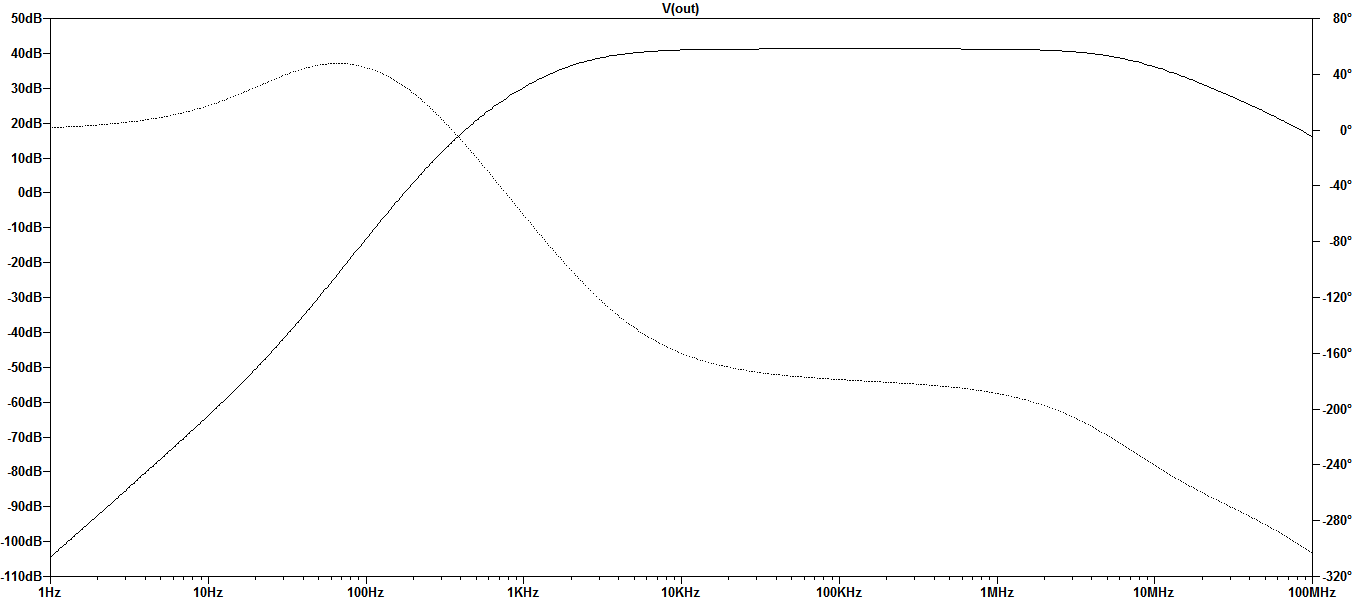
\includegraphics[scale=0.45]{../EJ2/rtaenfrec}
\caption{Simulaci\'on del circuito \ref{circ2}}
\label{simEj2}
\end{figure}

En la simulaci\'on de la figura \ref{simEj2}, la l\'inea oscura corresponde al m\'odulo de la funci\'on transferencia, mientras que la clara corresponde a su fase. 

\subsection*{\color{orange} Comparaci\'on entre el c\'alculo y la simulaci\'on de la funci\'on transferencia}

A partir de la l\'inea oscura del diagrama de Bode de la figura \ref{simEj2} (que corresponde al m\'odulo de la ganancia en dB), se puede ver que a bajas frecuencias coincide con  el valor obtenido en la ecuaci\'on \ref{ec2}. Esta comparaci\'on la hacemos a bajas frecuencias, ya que el c\'alculo de la funci\'on transferencia, con el cu\'al se obtuvo que la ganancia es de -112dB, surge de modelar un circuito equivalente del circuito \ref{circ2} para pequeña señal. Esto es, a bajas frecuencias, donde los capacitores se comportan como un cable.




















